\documentclass[12pt]{article}
\usepackage{natbib}
\usepackage[margin=1in]{geometry}
\usepackage{graphicx}
\usepackage{placeins}
\usepackage{titlesec}
\usepackage{float}
\titleformat*{\section}{\large\bfseries}
\begin{document}
		\title{Ethical Case Study: \\Texas City Refinery Explosion}

	\author{Duy Duong\\UID: 505183737\\Discussion 1B\\xxx words}
	\maketitle
	
	\begin{abstract}
Placeholder
	\end{abstract}
	\setlength{\parskip}{1em}
	\section*{Problem statement}
	
	\section*{Background}
	
	On March 23, 2005, an oil refinery in Texas City, owned by British Petroleum (BP), exploded and killed 15 people, injuring 170 more. The plant was built in 1934 and acquired by BP in 1999, at which point it had already fallen out of use for many years, with many crucial safety upgrades postponed by its previous owner (cite PBS). Part of maintenance work BP planned to do with the plant include the ISOM, which converted low octane hydrocarbons (organic compounds of hydrogen and carbon) into high octane ones that can be blended into unleaded gasoline. This process required the use of a raffinate splitter - a tower that separates light hydrocarbon components from heavy ones (such as octane), shown in Figure \ref{fig:ISOMunit}. After the hydrocarbons are split, they travel in 3 directions: the heavy and light hydrocarbons are pumped to the heavy and light raff storage tank respectively, and the hot vapors travel to the blowdown drum, which acted as a cooler and waste disposal unit for these gases.
	
	\begin{figure}[H]

		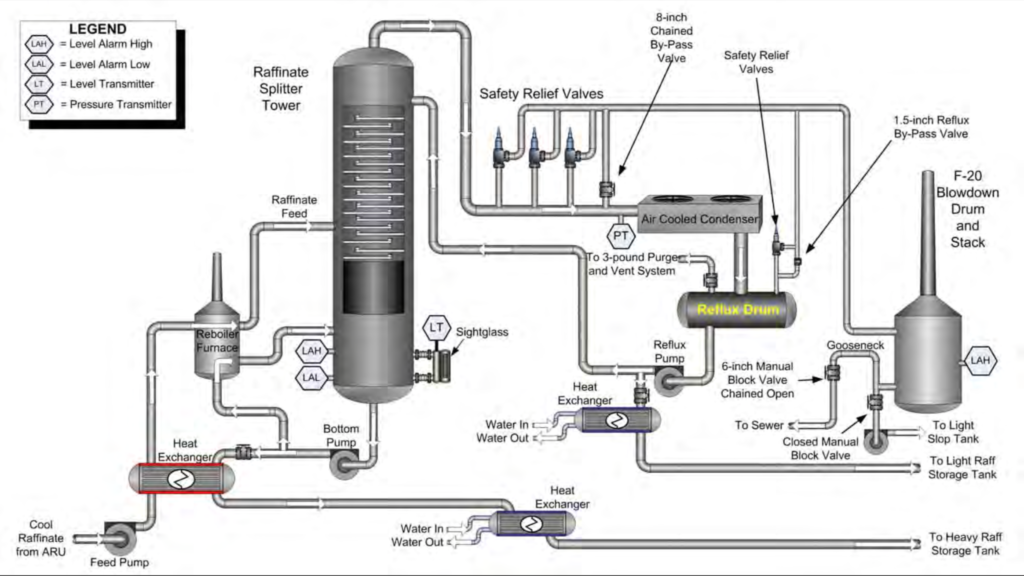
\includegraphics[width=\textwidth]{BP_Texas_City_ISOM_unit.png}
		\caption{Flow diagram of the ISOM unit. (cite BP report)}
		\label{fig:ISOMunit}
	\end{figure}
	
	The raffinate splitter, in normal operation, would have around 2m of liquid from its base. This liquid level was controlled by many overlapping safety systems, all of which had one or more major issues that were not acknowledged nor resolved even after a damning safety report by consulting firm Telos earlier that year (cite Telos report). On the day of the accident, the heavy storage tank was nearly full from the previous night's operation and the level control valve was shut off, cutting the downward flow to the heavy tank. When the raffine splitter was filled the next morning, the liquid level went up many times the safe amount as there was nowhere else for the materials to go. The raffinate splitter tower overflowed when the liquids expand due to the heat during operation, sending liquid hydrocarbons to the blowdown drum, as seen in Figure \ref{fig:incidentdiagram}. As the blowdown drum inevitably overflowed as well, hot liquid hydrocarbons shot off from the top and flowed through the drain pipes for sewer disposal.
	
	\begin{figure}[H]

		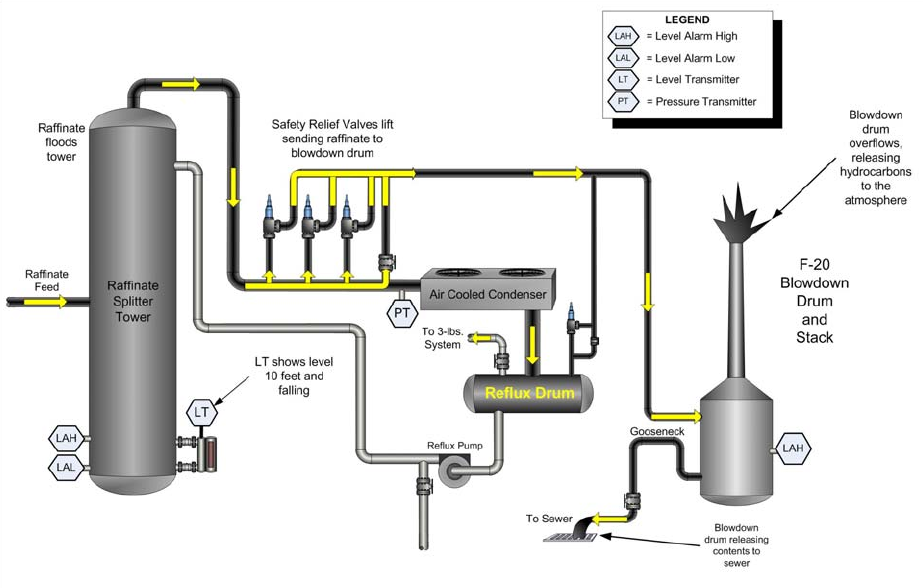
\includegraphics[width=\textwidth]{BP_Texas_City_incident_diagram.png}
		\caption{Incident diagram of the explosion. (cite BP report)}
		\label{fig:incidentdiagram}
	\end{figure}
	In the immediate vicinity were workers working on other parts of the ISOM, with their trailers parking right beside the plant, less than 110m away. The closest trailer was only 45m away from the blowdown drum. When the hot liquid hydrocarbons came out of the blowdown drum, the resulting vapor cloud consisting of highly flammable hydrocarbon fumes caused an idle truck engine to overheat and sparked a fire, igniting the vapor cloud. 
	
	The result was a massive explosion that completely destroyed most of the trailers, killing 15 instantly and injuring 180 more, mostly in the trailer areas. The explosion shattered windows three quarters of a mile away and damaged tanks holding hazardous materials such as benzene, leaking them to the environment. The subsequent fire burned up to 19000 $m^2$ of the refinery, causing damages in the millions of dollars. The ISOM itself did not return to normal operation until two years later after sustaining severe damages in the fire. (cite CBS)
	
	The disaster's impact is still felt years after the accident. A study conducted during and after the incident showed that it had led to a decline in the perceived mental and physical health of the people living in the area (cite BMJ). Lawsuits from the victims' families have followed BP, and they have had to pay out 1.6 billion USD in compensation. One notable lawsuit was Eva Rowe's, who demanded justice be brought on the company and forced them to release internal documents showing that they had prior knowledge of the issues plaguing the ISOM. 

	\section*{Engineering failure}
	\section*{Ethical analysis}
	\section*{Recommendations}
	\section*{Conclusion}
	\section*{Sources}
	https://www.pbs.org/wgbh/pages/frontline/the-spill/bp-troubled-past/
	https://www.csb.gov/bp-america-refinery-explosion/
	https://people.uvawise.edu/pww8y/Supplement/-ConceptsSup/Work/WkAccidents/BPTxCityFinalReport.pdf
	https://www.nytimes.com/2010/07/13/business/energy-environment/13bprisk.html?pagewanted=all
	https://www.propublica.org/article/blast-at-bp-texas-refinery-in-05-foreshadowed-gulf-disaster
	https://bloximages.newyork1.vip.townnews.com/galvnews.com/content/tncms/assets/v3/editorial/6/cb/6cb6d830-d239-11e4-9afa-2f2f90912f92/5511818abc022.pdf.pdf
	https://www.nytimes.com/2009/10/31/business/31labor.html
	https://jech.bmj.com/content/62/2/106
\end{document}